%% Paper D: are explanations less reliable when the model is wrong?
%% Target: Tecnologia en Marcha, special issue on Artificial Intelligence (deadline
%% 2026-10-15). See docs/reports/paper_d/README.md and ANALYSIS_PLAN.md.
%%
%% THIS IS THE SOURCE. paper_d.tex is GENERATED from it by scripts/pubs/render_paper_d.py,
%% which replaces every placeholder (table, key and format between double angle brackets,
%% syntax in the script's docstring) with the value in
%% outputs/analysis/paper_d/<table>.csv and registers each printed number in
%% pub/claim_registry.toml (RCA-001). Edit this file, never paper_d.tex.
%%
%% The journal takes Microsoft Word: letter, one column, Times 12 pt, 1.5 line spacing,
%% 5-15 pages, IEEE references, English and Spanish titles, abstracts and keywords.
%% This source is set to the same page so the PDF predicts the Word length;
%% scripts/pubs/build_paper_d.py renders the PDF and the .docx.
%%
%% Review is double-blind. The default build omits author identity; the full build
%% (author block, repository URL) is made by defining \fullversion before this file.
\documentclass[12pt,letterpaper]{article}
\usepackage[margin=25mm]{geometry}
\usepackage{fontspec}
\setmainfont{texgyretermes}[Extension=.otf, UprightFont=*-regular, BoldFont=*-bold,
  ItalicFont=*-italic, BoldItalicFont=*-bolditalic]
\usepackage{setspace}
\onehalfspacing
\usepackage{amsmath}
\usepackage{amssymb}
\usepackage{graphicx}
\usepackage{booktabs}
\usepackage{array}
\usepackage[hidelinks]{hyperref}
\usepackage{cite}
\setlength{\emergencystretch}{3em}

\newif\iffull
\ifdefined\fullversion \fulltrue \else \fullfalse \fi

\begin{document}

\begin{center}
{\large\bfseries Are explanations less reliable when the model is wrong? Post-hoc
explanation quality on misclassified instances\par}
\medskip
{\large\bfseries {\textquestiondown}Son menos fiables las explicaciones cuando el modelo se
equivoca? Calidad de las explicaciones post hoc en instancias mal clasificadas\par}
\medskip
\iffull
Jonathan Herrera-V\'asquez\par
{[}AUTHOR: profession{]}. Department of Computer Science, Universidad Americana de Europa
(UNADE), Canc\'un, Quintana Roo, Mexico.\par
jonnabio@gmail.com \quad ORCID: [AUTHOR: ORCID]
\else
\textit{Author information omitted for double-blind review.}
\fi
\end{center}

\section*{Abstract}
Explanations of machine-learning predictions are consulted most when a prediction is in
doubt, yet explainers are evaluated on averages over all instances. We ask whether
post-hoc explanations are less reliable when the model is wrong. Using an existing
benchmark on the UCI Adult data, we compare fidelity, stability and faithfulness gap
between correctly and incorrectly classified instances for SHAP, LIME, Anchors and DiCE
across five model families, with the run as the unit of analysis
(<<data:runs_analysed:d>> runs, <<data:analysed_total:int>> explained instances), Wilcoxon
signed-rank tests with Holm correction, a control for the prediction margin, and an
external check on German Credit. Explanations were less stable on misclassified instances
for all four explainers, and the deficit was large for SHAP (median difference
<<rq1:shap.stability.median:s3>>, $d_z =$ <<rq1:shap.stability.dz:s2>>) and DiCE
(<<rq1:dice.stability.median:s3>>, $d_z =$ <<rq1:dice.stability.dz:s2>>). The prediction
margin explained most of the DiCE deficit but not the SHAP deficit. Holding the margin
fixed, the features that SHAP, LIME and Anchors ranked first carried less of the
prediction on errors. Fidelity changed little and in opposite directions across
explainers. The pattern depended on the model family, and on German Credit it held for
Anchors but not for SHAP stability. Quality reported as an average can therefore
overstate how far an explanation of a wrong prediction should be trusted; audits should
report explanation quality separately for correct and incorrect predictions.

\noindent\textbf{Keywords:} explainable artificial intelligence; post-hoc explanations;
misclassification; explanation reliability; SHAP; LIME.

\section*{Resumen}
Las explicaciones de las predicciones de aprendizaje autom\'atico se consultan sobre todo
cuando una predicci\'on es dudosa, pero los explicadores se eval\'uan con promedios sobre
todas las instancias. Nos preguntamos si las explicaciones post hoc son menos fiables
cuando el modelo se equivoca. Con un banco de pruebas existente sobre UCI Adult,
comparamos fidelidad, estabilidad y brecha de borrado entre instancias bien y mal
clasificadas para SHAP, LIME, Anchors y DiCE en cinco familias de modelos, con la
ejecuci\'on como unidad de an\'alisis (<<data:runs_analysed:d>> ejecuciones,
<<data:analysed_total:int>> instancias), pruebas de Wilcoxon con correcci\'on de Holm,
un control del margen de predicci\'on y una verificaci\'on externa con German Credit.
Las explicaciones fueron menos estables en las
instancias mal clasificadas para los cuatro explicadores, y el d\'eficit fue grande para
SHAP (diferencia mediana <<rq1:shap.stability.median:s3>>,
$d_z =$ <<rq1:shap.stability.dz:s2>>) y DiCE (<<rq1:dice.stability.median:s3>>,
$d_z =$ <<rq1:dice.stability.dz:s2>>). El margen de predicci\'on explic\'o la mayor parte
del d\'eficit de DiCE, pero no el de SHAP. Con el margen fijo, las variables que SHAP, LIME
y Anchors situaron en primer lugar sostuvieron una parte menor de la predicci\'on en los
errores. El patr\'on dependi\'o de la familia de modelos y, en German Credit, se mantuvo
para Anchors pero no para la estabilidad de SHAP. La calidad promedio puede exagerar la
confianza que merece la explicaci\'on de una predicci\'on err\'onea; las auditor\'ias
deber\'ian informarla por separado para predicciones correctas e incorrectas.

\noindent\textbf{Palabras clave:} inteligencia artificial explicable; explicaciones post
hoc; errores de clasificaci\'on; fiabilidad de las explicaciones; SHAP; LIME.

\section{Introduction}

Post-hoc explainers such as SHAP \cite{lundberg2017unified}, LIME \cite{ribeiro2016why},
Anchors \cite{ribeiro2018anchors} and DiCE \cite{mothilal2020dice} are the usual way to
make the predictions of an opaque classifier inspectable \cite{adadi2018xai}. Their
quality is assessed with proxy metrics: whether the features an explanation ranks as
important are those that move the prediction (fidelity and deletion tests
\cite{bhatt2020evaluating,samek2017evaluating,hooker2019benchmark}), and whether similar
inputs receive similar explanations (stability \cite{alvarezmelis2018robustness}). These
metrics are reported as averages over a sample of instances, and benchmarks compare
explainers by those averages \cite{herrera2026framework}.

An average hides how quality is distributed across instances, and one split matters more
than most: whether the model's prediction was right. An explanation is rarely consulted to
confirm an obviously correct decision. It is consulted when a decision is contested, when
an auditor examines a failure, or when a user must decide whether to accept a
recommendation. In those situations the prediction is disproportionately likely to be
wrong. User studies show that explanations can raise acceptance of a model's
recommendation whether or not the recommendation is correct \cite{bansal2021whole}, and
explanations can be unreliable in ways that their appearance does not reveal
\cite{adebayo2018sanity,slack2020fooling}. If explanations are also less faithful or less
stable on misclassified instances, an explanation can look convincing exactly where it
deserves the least trust \cite{rudin2019stop,jacovi2020faithfulness}.

Whether explanation quality differs between correct and incorrect predictions is an
empirical question, and the usual reporting cannot answer it. We answer it with a
pre-specified re-analysis of an existing benchmark that explained, under one protocol,
balanced samples of true positives, true negatives, false positives and false negatives
for four explainers and five model families. We ask four questions:
\begin{itemize}
\item \textbf{RQ1.} Does explanation quality differ between correctly and incorrectly
classified instances, for each explainer?
\item \textbf{RQ2.} Does the difference depend on the model family?
\item \textbf{RQ3.} Among errors, do false positives and false negatives differ?
\item \textbf{RQ4.} Is the difference explained by proximity to the decision boundary?
Errors tend to lie near it, and some metrics may depend on the margin rather than on
correctness itself.
\end{itemize}
The contribution is an instance-level answer, with the run as the unit of inference, a
margin control, an external check on a second dataset, and a practical recommendation
for how explanation audits should report quality.

\section{Materials and methods}

\subsection{Benchmark and data}

The data are the runs of an existing benchmark of post-hoc explainers on the UCI Adult
income data \cite{kohavi1996scaling,becker1996adult}, released with its protocol and
reproducibility contract in \cite{herrera2026framework}. That study, and a later
analysis of the same runs, compare explainers by their average quality over all
instances. The present analysis is different and reports none of their results: it
compares each explainer with itself, between correct and misclassified instances of the
same run. Re-using the cohort rather than re-executing it keeps the explainers, models and
instances fixed, so the only contrast is the correctness of the prediction.

Five classifiers, each trained once, were explained: logistic regression,
random forest \cite{breiman2001random}, gradient-boosted trees (XGBoost)
\cite{chen2016xgboost}, a support vector machine and a multilayer perceptron. Each run
crossed one model family with one explainer, one random seed (42, 123, 456, 789 or 999)
and one sampling intensity of $n = 50$, $100$ or $200$ instances per error quadrant. The
seed fixed the partition from which instances were drawn; the models were trained on the
partition of seed 42. Within a run, test instances
were sampled separately from the four quadrants (TP, TN, FP, FN), so correct and
misclassified instances are represented in nearly equal numbers by design.

Of the <<data:runs_total:d>> run files, <<data:runs_analysed:d>> entered the analysis.
Anchors and DiCE produced no explanations in
<<data:anchors.runs_present-anchors.runs_nonempty:d>> and
<<data:dice.runs_present-dice.runs_nonempty:d>> runs respectively (failed or
non-converged), and <<data:shap.runs_nonempty-shap.runs_analysed:d>> SHAP runs had fewer
than ten instances in one of the two groups. The analysis covers
<<data:analysed_total:int>> explained instances; <<data:unlabelled_total:d>> instances
without a recorded quadrant were excluded. Table~\ref{tab:data} gives the counts per
explainer.

\begin{table}[ht]
\centering
\caption{Runs and instances analysed per explainer (UCI Adult).}
\label{tab:data}
\begin{tabular}{lrrrr}
\toprule
Explainer & Runs present & Runs analysed & Correct & Misclassified \\
\midrule
SHAP & <<data:shap.runs_present:d>> & <<data:shap.runs_analysed:d>> & <<data:shap.correct:int>> & <<data:shap.misclassified:int>> \\
LIME & <<data:lime.runs_present:d>> & <<data:lime.runs_analysed:d>> & <<data:lime.correct:int>> & <<data:lime.misclassified:int>> \\
Anchors & <<data:anchors.runs_present:d>> & <<data:anchors.runs_analysed:d>> & <<data:anchors.correct:int>> & <<data:anchors.misclassified:int>> \\
DiCE & <<data:dice.runs_present:d>> & <<data:dice.runs_analysed:d>> & <<data:dice.correct:int>> & <<data:dice.misclassified:int>> \\
\bottomrule
\end{tabular}
\end{table}

For the external check we used the German Credit data \cite{hofmann1994statlog} from the
same benchmark: random forest and XGBoost, explained by SHAP and Anchors, three seeds
each (<<ext:runs_total:d>> runs). These runs have 13 to 37 errors per quadrant. A
third dataset in the benchmark, Breast Cancer, was excluded in advance because it has only
one to four errors per quadrant per run.

\subsection{Explainers and quality metrics}

SHAP used TreeExplainer for the tree models and KernelExplainer otherwise; LIME used a
tabular surrogate with ten features. Both return an attribution vector
$e(x) \in \mathbb{R}^{M}$ over the $M$ model features. Anchors returns a rule; it is
represented as a binary vector marking the features in the rule. DiCE returns a
counterfactual $x'$ of the opposite class, represented as $|x - x'|$. Let $f(x)$ be the
model's predicted probability of the positive class, and let masking feature $j$ replace
its value with the training mean. The metrics, computed per instance by the benchmark
\cite{herrera2026framework}, are:

\textbf{Stability} $S$ \cite{alvarezmelis2018robustness}: the explainer is run on $T$
copies of $x$ perturbed with Gaussian noise, and $S$ is the mean cosine similarity of the
resulting vectors over all pairs:
\begin{equation}
S = \frac{2}{T(T-1)} \sum_{a<b} \cos\left(e^{(a)}, e^{(b)}\right).
\end{equation}

\textbf{Fidelity} $F$, a single-feature form of faithfulness correlation
\cite{bhatt2020evaluating}: the Pearson correlation, across features, between the
magnitude of each attribution and the change in prediction when that feature alone is
masked:
\begin{equation}
F = \rho\left( \left\{ |e_j(x)| \right\}_{j=1}^{M},\ \left\{ |f(x) - f(\tilde{x}^{(j)})| \right\}_{j=1}^{M} \right).
\end{equation}

\textbf{Faithfulness gap} $G$, a deletion test \cite{samek2017evaluating,hooker2019benchmark}:
the change in prediction when the $k = 5$ features with the largest attributions are
masked together:
\begin{equation}
G = \left| f(x) - f\left(\tilde{x}^{(\text{top-}k)}\right) \right|.
\end{equation}

\textbf{Sparsity}, the share of features with a non-negligible attribution, was analysed
as a secondary metric. Explanation time was summarised descriptively. For all three primary
metrics, higher values indicate a better explanation.

\subsection{Statistical analysis}

The analysis plan, with the questions, metrics, tests and corrections, was written and
committed to the project repository before any result was computed; its two deviations
are reported below. Instances are nested in runs, so instance-level tests would treat
thousands of dependent explanations as independent. The run is therefore the unit of
inference. For run $r$ and metric $Q$,
\begin{equation}
\Delta_r = \bar{Q}_{r,\mathrm{mis}} - \bar{Q}_{r,\mathrm{cor}},
\end{equation}
the mean over misclassified instances (FP and FN) minus the mean over correct instances
(TP and TN). A negative $\Delta$ means lower quality on errors.

\textbf{RQ1:} for each explainer and primary metric (12 tests), a two-sided Wilcoxon
signed-rank test of $\Delta = 0$ across runs \cite{wilcoxon1945individual}, with Holm
correction across the 12 tests \cite{holm1979simple} at $\alpha = 0.05$. We report the
median $\Delta$, the mean with a 95\% confidence interval, and the standardised effect
$d_z$ (mean over standard deviation of $\Delta$) \cite{lakens2013calculating}. An effect
is called practically relevant when it is significant after correction, $|d_z| \geq 0.5$
and $|\text{median}\ \Delta| \geq 0.05$. As a robustness check, the analysis was repeated
after averaging $\Delta$ over the three sampling intensities within each model and seed.
\textbf{RQ2:} $\Delta$ by model family, with a Kruskal--Wallis test
\cite{kruskal1952use} per explainer and metric (Holm across 12). \textbf{RQ3:} as RQ1 with
$\Delta_r = \bar{Q}_{r,\mathrm{FP}} - \bar{Q}_{r,\mathrm{FN}}$.

\textbf{RQ4:} misclassified instances lie closer to the decision boundary, and metrics
that perturb or mask the input may behave differently there. The margin of an instance,
$m = |\hat{p} - 0.5|$, was recomputed from the stored models. For each explainer and
metric we fitted, at instance level,
\begin{equation}
Q_{ir} = \alpha_r + \beta\, \mathrm{mis}_{ir} + \gamma\, m_{ir} + \varepsilon_{ir},
\end{equation}
with run fixed effects $\alpha_r$ and standard errors clustered by run
\cite{cameron2015practitioner}, and compared $\beta$ with its value when the margin is
omitted. A difference is called explained by the margin when $\beta$ shrinks by more than
half and its confidence interval includes zero. The external check repeats RQ1 on German
Credit descriptively: with six runs per explainer, no test can reach significance after
correction.

\textbf{Deviations from the plan.} (1) For the random-forest runs executed first, the stored
model reproduced only part of the recorded predictions, so their margin cannot be
recomputed; RQ4 therefore uses the <<rq4:runs_reproducible:d>> of
<<rq4:runs_nonempty:d>> runs whose recorded predictions the stored model reproduces
(at least 99\%), which leaves <<rq4:rf.runs_reproducible:d>> of
<<rq4:rf.runs_nonempty:d>> random-forest runs. RQ1--RQ3 are unaffected, because their
correct and misclassified labels were assigned by the model that actually ran. (2) For the
SVM, $\hat{p}$ is the Platt-scaled probability \cite{platt1999probabilistic}, which
disagrees with the predicted class for <<rq4:svm.proba_pred_disagree:d>> of
<<rq4:svm.proba_total:int>> instances; they were kept.

\section{Results}

\subsection{Correct versus misclassified instances (RQ1)}

Table~\ref{tab:rq1} and Figure~\ref{fig:rq1} give the per-run differences. Stability was
lower on misclassified instances for all four explainers after correction. The deficit
was large for SHAP, lower in all <<rq1:shap.stability.neg:d>> runs (median
<<rq1:shap.stability.median:s3>>, $d_z =$ <<rq1:shap.stability.dz:s2>>), and for DiCE,
lower in <<rq1:dice.stability.neg:d>> of <<rq1:dice.stability.n:d>> runs (median
<<rq1:dice.stability.median:s3>>, $d_z =$ <<rq1:dice.stability.dz:s2>>). For LIME the
deficit was consistent, lower in <<rq1:lime.stability.neg:d>> of
<<rq1:lime.stability.n:d>> runs, but small in absolute terms
(median <<rq1:lime.stability.median:s4>>), because LIME's stability on these data is
close to zero on average. For Anchors the median was close to zero.

Fidelity moved in opposite directions. It was lower on errors for DiCE (median
<<rq1:dice.fidelity.median:s3>>) and Anchors (<<rq1:anchors.fidelity.median:s3>>),
higher for LIME (<<rq1:lime.fidelity.median:s3>>), and not significantly different for
SHAP after correction ($p_{\mathrm{Holm}} =$ <<rq1:shap.fidelity.p_holm:p>>). The
faithfulness gap was lower on errors for SHAP (median
<<rq1:shap.faithfulness_gap.median:s3>>, lower in <<rq1:shap.faithfulness_gap.neg:d>>
of <<rq1:shap.faithfulness_gap.n:d>> runs) and DiCE, and did not differ for LIME and
Anchors. Of the 12 primary tests, <<rq1:n_significant:d>> were significant after
correction and <<rq1:n_relevant:d>> met the practical-relevance criterion: SHAP stability,
DiCE stability and DiCE fidelity. The robustness analysis over model--seed units agreed in
direction and significance for <<rq1r:n_agree:d>> of the 12 tests; the exceptions were the
LIME faithfulness gap, not significant in either analysis, and the DiCE faithfulness gap,
which lost significance.

\begin{table}[ht]
\centering
\caption{Per-run difference in quality, misclassified minus correct instances (UCI Adult).
$n$: runs; CI: 95\% confidence interval of the mean; $p_{\mathrm{Holm}}$: Wilcoxon
signed-rank, Holm-corrected within the 12 primary and, separately, the 4 sparsity tests.}
\label{tab:rq1}
\small
\begin{tabular}{llrrrrr}
\toprule
Metric & Explainer & $n$ & Median $\Delta$ & Mean $\Delta$ [95\% CI] & $d_z$ & $p_{\mathrm{Holm}}$ \\
\midrule
Stability & SHAP & <<rq1:shap.stability.n:d>> & <<rq1:shap.stability.median:s3>> & <<rq1:shap.stability.mean:s3>> [<<rq1:shap.stability.ci_lo:s3>>, <<rq1:shap.stability.ci_hi:s3>>] & <<rq1:shap.stability.dz:s2>> & <<rq1:shap.stability.p_holm:p>> \\
 & LIME & <<rq1:lime.stability.n:d>> & <<rq1:lime.stability.median:s3>> & <<rq1:lime.stability.mean:s3>> [<<rq1:lime.stability.ci_lo:s3>>, <<rq1:lime.stability.ci_hi:s3>>] & <<rq1:lime.stability.dz:s2>> & <<rq1:lime.stability.p_holm:p>> \\
 & Anchors & <<rq1:anchors.stability.n:d>> & <<rq1:anchors.stability.median:s3>> & <<rq1:anchors.stability.mean:s3>> [<<rq1:anchors.stability.ci_lo:s3>>, <<rq1:anchors.stability.ci_hi:s3>>] & <<rq1:anchors.stability.dz:s2>> & <<rq1:anchors.stability.p_holm:p>> \\
 & DiCE & <<rq1:dice.stability.n:d>> & <<rq1:dice.stability.median:s3>> & <<rq1:dice.stability.mean:s3>> [<<rq1:dice.stability.ci_lo:s3>>, <<rq1:dice.stability.ci_hi:s3>>] & <<rq1:dice.stability.dz:s2>> & <<rq1:dice.stability.p_holm:p>> \\
\midrule
Fidelity & SHAP & <<rq1:shap.fidelity.n:d>> & <<rq1:shap.fidelity.median:s3>> & <<rq1:shap.fidelity.mean:s3>> [<<rq1:shap.fidelity.ci_lo:s3>>, <<rq1:shap.fidelity.ci_hi:s3>>] & <<rq1:shap.fidelity.dz:s2>> & <<rq1:shap.fidelity.p_holm:p>> \\
 & LIME & <<rq1:lime.fidelity.n:d>> & <<rq1:lime.fidelity.median:s3>> & <<rq1:lime.fidelity.mean:s3>> [<<rq1:lime.fidelity.ci_lo:s3>>, <<rq1:lime.fidelity.ci_hi:s3>>] & <<rq1:lime.fidelity.dz:s2>> & <<rq1:lime.fidelity.p_holm:p>> \\
 & Anchors & <<rq1:anchors.fidelity.n:d>> & <<rq1:anchors.fidelity.median:s3>> & <<rq1:anchors.fidelity.mean:s3>> [<<rq1:anchors.fidelity.ci_lo:s3>>, <<rq1:anchors.fidelity.ci_hi:s3>>] & <<rq1:anchors.fidelity.dz:s2>> & <<rq1:anchors.fidelity.p_holm:p>> \\
 & DiCE & <<rq1:dice.fidelity.n:d>> & <<rq1:dice.fidelity.median:s3>> & <<rq1:dice.fidelity.mean:s3>> [<<rq1:dice.fidelity.ci_lo:s3>>, <<rq1:dice.fidelity.ci_hi:s3>>] & <<rq1:dice.fidelity.dz:s2>> & <<rq1:dice.fidelity.p_holm:p>> \\
\midrule
Faithfulness & SHAP & <<rq1:shap.faithfulness_gap.n:d>> & <<rq1:shap.faithfulness_gap.median:s3>> & <<rq1:shap.faithfulness_gap.mean:s3>> [<<rq1:shap.faithfulness_gap.ci_lo:s3>>, <<rq1:shap.faithfulness_gap.ci_hi:s3>>] & <<rq1:shap.faithfulness_gap.dz:s2>> & <<rq1:shap.faithfulness_gap.p_holm:p>> \\
gap & LIME & <<rq1:lime.faithfulness_gap.n:d>> & <<rq1:lime.faithfulness_gap.median:s3>> & <<rq1:lime.faithfulness_gap.mean:s3>> [<<rq1:lime.faithfulness_gap.ci_lo:s3>>, <<rq1:lime.faithfulness_gap.ci_hi:s3>>] & <<rq1:lime.faithfulness_gap.dz:s2>> & <<rq1:lime.faithfulness_gap.p_holm:p>> \\
 & Anchors & <<rq1:anchors.faithfulness_gap.n:d>> & <<rq1:anchors.faithfulness_gap.median:s3>> & <<rq1:anchors.faithfulness_gap.mean:s3>> [<<rq1:anchors.faithfulness_gap.ci_lo:s3>>, <<rq1:anchors.faithfulness_gap.ci_hi:s3>>] & <<rq1:anchors.faithfulness_gap.dz:s2>> & <<rq1:anchors.faithfulness_gap.p_holm:p>> \\
 & DiCE & <<rq1:dice.faithfulness_gap.n:d>> & <<rq1:dice.faithfulness_gap.median:s3>> & <<rq1:dice.faithfulness_gap.mean:s3>> [<<rq1:dice.faithfulness_gap.ci_lo:s3>>, <<rq1:dice.faithfulness_gap.ci_hi:s3>>] & <<rq1:dice.faithfulness_gap.dz:s2>> & <<rq1:dice.faithfulness_gap.p_holm:p>> \\
\midrule
Sparsity & SHAP & <<rq1:shap.sparsity.n:d>> & <<rq1:shap.sparsity.median:s3>> & <<rq1:shap.sparsity.mean:s3>> [<<rq1:shap.sparsity.ci_lo:s3>>, <<rq1:shap.sparsity.ci_hi:s3>>] & <<rq1:shap.sparsity.dz:s2>> & <<rq1:shap.sparsity.p_holm:p>> \\
 & LIME & <<rq1:lime.sparsity.n:d>> & <<rq1:lime.sparsity.median:s3>> & <<rq1:lime.sparsity.mean:s3>> [<<rq1:lime.sparsity.ci_lo:s3>>, <<rq1:lime.sparsity.ci_hi:s3>>] & <<rq1:lime.sparsity.dz:s2>> & <<rq1:lime.sparsity.p_holm:p>> \\
 & Anchors & <<rq1:anchors.sparsity.n:d>> & <<rq1:anchors.sparsity.median:s3>> & <<rq1:anchors.sparsity.mean:s3>> [<<rq1:anchors.sparsity.ci_lo:s3>>, <<rq1:anchors.sparsity.ci_hi:s3>>] & <<rq1:anchors.sparsity.dz:s2>> & <<rq1:anchors.sparsity.p_holm:p>> \\
 & DiCE & <<rq1:dice.sparsity.n:d>> & <<rq1:dice.sparsity.median:s3>> & <<rq1:dice.sparsity.mean:s3>> [<<rq1:dice.sparsity.ci_lo:s3>>, <<rq1:dice.sparsity.ci_hi:s3>>] & <<rq1:dice.sparsity.dz:s2>> & <<rq1:dice.sparsity.p_holm:p>> \\
\bottomrule
\end{tabular}
\end{table}

\begin{figure}[ht]
\centering
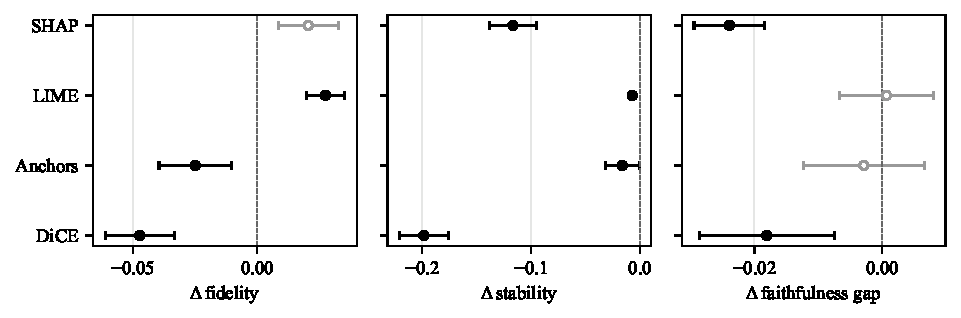
\includegraphics[width=\linewidth]{figures/fig1}
\caption{Mean per-run difference in quality between misclassified and correct instances,
with 95\% confidence intervals (UCI Adult). Filled markers: significant after Holm
correction; open markers: not significant. Negative values mean lower quality on errors.}
\label{fig:rq1}
\end{figure}

Sparsity differed little in absolute terms (all medians within
$\pm<<rq1:dice.sparsity.median:u4>>$ of zero apart from Anchors). Explanation time did
not differ systematically, except for Anchors, which took a median
<<rq1:anchors.cost.median:int>> ms longer per instance on errors, plausibly because its rule
search runs longer near the boundary.

\subsection{Differences across model families (RQ2)}

The size, and for fidelity and the faithfulness gap also the sign, of the difference
depended on the model family (Figure~\ref{fig:rq2}). The Kruskal--Wallis test was
significant after correction for <<rq2:n_kw_significant:d>> of the
<<rq2:n_kw_tests:d>> explainer--metric combinations; the two exceptions were the
stability of LIME and Anchors, whose differences were small for every family. The SHAP
stability deficit was largest for the multilayer perceptron (median
<<rq2:shap.stability.mlp.median:s3>>) and XGBoost (<<rq2:shap.stability.xgb.median:s3>>)
and smallest for the random forest (<<rq2:shap.stability.rf.median:s3>>) and the SVM
(<<rq2:shap.stability.svm.median:s3>>). The DiCE
stability deficit was present for every family and largest for logistic regression
(<<rq2:dice.stability.logreg.median:s3>>).

\begin{figure}[ht]
\centering
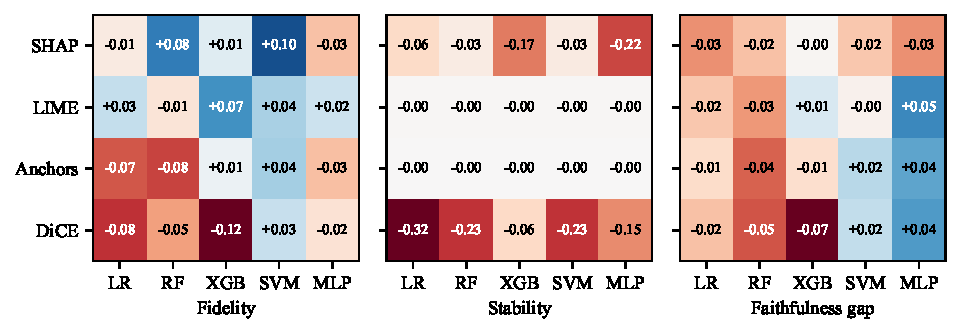
\includegraphics[width=\linewidth]{figures/fig2}
\caption{Median per-run difference (misclassified minus correct) by explainer and model
family. LR: logistic regression; RF: random forest; XGB: XGBoost; SVM: support vector
machine; MLP: multilayer perceptron. Red: lower quality on errors; blue: higher.}
\label{fig:rq2}
\end{figure}

\subsection{False positives versus false negatives (RQ3)}

Among errors, the faithfulness gap was much larger for false positives than for false
negatives for every explainer (Table~\ref{tab:rq3}); for SHAP and LIME this held in every
run. DiCE stability was lower on false positives. The other differences were small.
A likely reason for the faithfulness-gap asymmetry is how the metric masks features:
masking to the training mean moves an instance towards the majority, negative class, so
removing the top features changes a positive prediction (a false positive) far more than a
negative one (a false negative). The gap is therefore not comparable across predicted classes, which
matters for any audit that compares explanations of different decisions.

\begin{table}[ht]
\centering
\caption{Per-run difference, false positives minus false negatives: median $\Delta$
($p_{\mathrm{Holm}}$, Wilcoxon signed-rank, Holm-corrected across the 12 tests).}
\label{tab:rq3}
\begin{tabular}{lccc}
\toprule
Explainer & Fidelity & Stability & Faithfulness gap \\
\midrule
SHAP & <<rq3:shap.fidelity.median:s3>> (<<rq3:shap.fidelity.p_holm:p>>) & <<rq3:shap.stability.median:s3>> (<<rq3:shap.stability.p_holm:p>>) & <<rq3:shap.faithfulness_gap.median:s3>> (<<rq3:shap.faithfulness_gap.p_holm:p>>) \\
LIME & <<rq3:lime.fidelity.median:s3>> (<<rq3:lime.fidelity.p_holm:p>>) & <<rq3:lime.stability.median:s3>> (<<rq3:lime.stability.p_holm:p>>) & <<rq3:lime.faithfulness_gap.median:s3>> (<<rq3:lime.faithfulness_gap.p_holm:p>>) \\
Anchors & <<rq3:anchors.fidelity.median:s3>> (<<rq3:anchors.fidelity.p_holm:p>>) & <<rq3:anchors.stability.median:s3>> (<<rq3:anchors.stability.p_holm:p>>) & <<rq3:anchors.faithfulness_gap.median:s3>> (<<rq3:anchors.faithfulness_gap.p_holm:p>>) \\
DiCE & <<rq3:dice.fidelity.median:s3>> (<<rq3:dice.fidelity.p_holm:p>>) & <<rq3:dice.stability.median:s3>> (<<rq3:dice.stability.p_holm:p>>) & <<rq3:dice.faithfulness_gap.median:s3>> (<<rq3:dice.faithfulness_gap.p_holm:p>>) \\
\bottomrule
\end{tabular}
\end{table}

\subsection{The role of the decision boundary (RQ4)}

Errors were indeed closer to the boundary (median margin
<<rq4:shap.stability.margin_median_mis:u2>> against <<rq4:shap.stability.margin_median_cor:u2>>
for correct instances in the SHAP runs), and stability rose with the margin for every
explainer (Figure~\ref{fig:rq4}). Controlling for the margin changed the picture in three
ways (Table~\ref{tab:rq4}). First, the DiCE stability deficit was almost entirely a
margin effect: its coefficient fell from <<rq4:dice.stability.b_raw:s3>> to
<<rq4:dice.stability.b_adj:s3>>, with a confidence interval including zero. A
counterfactual for an instance near the boundary needs only a small change, and small
changes vary more under noise. Second, the SHAP stability deficit was reduced but
remained: <<rq4:shap.stability.b_raw:s3>> without and <<rq4:shap.stability.b_adj:s3>>
[<<rq4:shap.stability.lo_adj:s3>>, <<rq4:shap.stability.hi_adj:s3>>] with the margin.
Figure~\ref{fig:rq4} shows the same: at equal margin, SHAP explanations of errors are less
stable than those of correct predictions. Third, the faithfulness gap, which in RQ1
was lower on errors only for SHAP and DiCE and by small amounts, became lower on errors once
the margin was held fixed for SHAP
(<<rq4:shap.faithfulness_gap.b_adj:s3>>), LIME (<<rq4:lime.faithfulness_gap.b_adj:s3>>)
and Anchors (<<rq4:anchors.faithfulness_gap.b_adj:s3>>). Near the boundary any deletion
moves the prediction a lot, which inflates the gap of errors; at equal margin, the
features named first carry less of an erroneous prediction. The fidelity differences
were largely margin effects: the LIME advantage on errors fell from
<<rq4:lime.fidelity.b_raw:s3>> to <<rq4:lime.fidelity.b_adj:s3>>, the Anchors deficit
vanished, and the DiCE deficit reversed sign.

\begin{table}[ht]
\centering
\caption{Coefficient of misclassification $\beta$ (95\% CI) in run fixed-effects
regressions, without and with the prediction margin; standard errors clustered by run.
Runs whose recorded predictions the stored model reproduces.}
\label{tab:rq4}
\small
\begin{tabular}{llcc}
\toprule
Metric & Explainer & $\beta$ without margin & $\beta$ with margin \\
\midrule
Stability & SHAP & <<rq4:shap.stability.b_raw:s3>> [<<rq4:shap.stability.lo_raw:s3>>, <<rq4:shap.stability.hi_raw:s3>>] & <<rq4:shap.stability.b_adj:s3>> [<<rq4:shap.stability.lo_adj:s3>>, <<rq4:shap.stability.hi_adj:s3>>] \\
 & LIME & <<rq4:lime.stability.b_raw:s3>> [<<rq4:lime.stability.lo_raw:s3>>, <<rq4:lime.stability.hi_raw:s3>>] & <<rq4:lime.stability.b_adj:s3>> [<<rq4:lime.stability.lo_adj:s3>>, <<rq4:lime.stability.hi_adj:s3>>] \\
 & Anchors & <<rq4:anchors.stability.b_raw:s3>> [<<rq4:anchors.stability.lo_raw:s3>>, <<rq4:anchors.stability.hi_raw:s3>>] & <<rq4:anchors.stability.b_adj:s3>> [<<rq4:anchors.stability.lo_adj:s3>>, <<rq4:anchors.stability.hi_adj:s3>>] \\
 & DiCE & <<rq4:dice.stability.b_raw:s3>> [<<rq4:dice.stability.lo_raw:s3>>, <<rq4:dice.stability.hi_raw:s3>>] & <<rq4:dice.stability.b_adj:s3>> [<<rq4:dice.stability.lo_adj:s3>>, <<rq4:dice.stability.hi_adj:s3>>] \\
\midrule
Fidelity & SHAP & <<rq4:shap.fidelity.b_raw:s3>> [<<rq4:shap.fidelity.lo_raw:s3>>, <<rq4:shap.fidelity.hi_raw:s3>>] & <<rq4:shap.fidelity.b_adj:s3>> [<<rq4:shap.fidelity.lo_adj:s3>>, <<rq4:shap.fidelity.hi_adj:s3>>] \\
 & LIME & <<rq4:lime.fidelity.b_raw:s3>> [<<rq4:lime.fidelity.lo_raw:s3>>, <<rq4:lime.fidelity.hi_raw:s3>>] & <<rq4:lime.fidelity.b_adj:s3>> [<<rq4:lime.fidelity.lo_adj:s3>>, <<rq4:lime.fidelity.hi_adj:s3>>] \\
 & Anchors & <<rq4:anchors.fidelity.b_raw:s3>> [<<rq4:anchors.fidelity.lo_raw:s3>>, <<rq4:anchors.fidelity.hi_raw:s3>>] & <<rq4:anchors.fidelity.b_adj:s3>> [<<rq4:anchors.fidelity.lo_adj:s3>>, <<rq4:anchors.fidelity.hi_adj:s3>>] \\
 & DiCE & <<rq4:dice.fidelity.b_raw:s3>> [<<rq4:dice.fidelity.lo_raw:s3>>, <<rq4:dice.fidelity.hi_raw:s3>>] & <<rq4:dice.fidelity.b_adj:s3>> [<<rq4:dice.fidelity.lo_adj:s3>>, <<rq4:dice.fidelity.hi_adj:s3>>] \\
\midrule
Faithfulness & SHAP & <<rq4:shap.faithfulness_gap.b_raw:s3>> [<<rq4:shap.faithfulness_gap.lo_raw:s3>>, <<rq4:shap.faithfulness_gap.hi_raw:s3>>] & <<rq4:shap.faithfulness_gap.b_adj:s3>> [<<rq4:shap.faithfulness_gap.lo_adj:s3>>, <<rq4:shap.faithfulness_gap.hi_adj:s3>>] \\
gap & LIME & <<rq4:lime.faithfulness_gap.b_raw:s3>> [<<rq4:lime.faithfulness_gap.lo_raw:s3>>, <<rq4:lime.faithfulness_gap.hi_raw:s3>>] & <<rq4:lime.faithfulness_gap.b_adj:s3>> [<<rq4:lime.faithfulness_gap.lo_adj:s3>>, <<rq4:lime.faithfulness_gap.hi_adj:s3>>] \\
 & Anchors & <<rq4:anchors.faithfulness_gap.b_raw:s3>> [<<rq4:anchors.faithfulness_gap.lo_raw:s3>>, <<rq4:anchors.faithfulness_gap.hi_raw:s3>>] & <<rq4:anchors.faithfulness_gap.b_adj:s3>> [<<rq4:anchors.faithfulness_gap.lo_adj:s3>>, <<rq4:anchors.faithfulness_gap.hi_adj:s3>>] \\
 & DiCE & <<rq4:dice.faithfulness_gap.b_raw:s3>> [<<rq4:dice.faithfulness_gap.lo_raw:s3>>, <<rq4:dice.faithfulness_gap.hi_raw:s3>>] & <<rq4:dice.faithfulness_gap.b_adj:s3>> [<<rq4:dice.faithfulness_gap.lo_adj:s3>>, <<rq4:dice.faithfulness_gap.hi_adj:s3>>] \\
\bottomrule
\end{tabular}
\end{table}

\begin{figure}[ht]
\centering
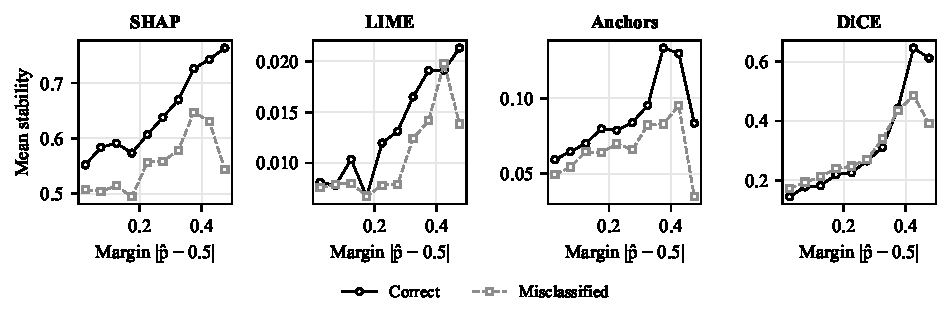
\includegraphics[width=\linewidth]{figures/fig3}
\caption{Mean stability by prediction margin $|\hat{p} - 0.5|$ for correct and
misclassified instances (UCI Adult; bins of width 0.05 with at least 30 instances).}
\label{fig:rq4}
\end{figure}

\subsection{External check on German Credit}

On German Credit, Anchors reproduced the Adult pattern: fidelity and faithfulness gap were
lower on errors in all six runs (medians <<ext:anchors.fidelity.median:s3>> and
<<ext:anchors.faithfulness_gap.median:s3>>) and stability in five
(<<ext:anchors.stability.median:s3>>). SHAP did not: its stability was higher on errors
in <<ext:shap.stability.pos:d>> of six runs (median <<ext:shap.stability.median:s3>>),
while its fidelity was lower in all six (<<ext:shap.fidelity.median:s3>>). With six runs
these are descriptive. They show that the size, and for SHAP the direction, of the
difference depends on the data as well as on the model.

\section{Discussion}

The answer to the title question is a qualified yes. On the Adult benchmark, explanations
of wrong predictions were less stable for every explainer, and for SHAP and DiCE the
difference was large: a SHAP explanation of a misclassified instance is markedly more
sensitive to small input noise than one of a correct prediction. Averages over all
instances hide this, because correct and incorrect predictions are pooled. Because the
benchmark sampled the four quadrants in balance, the pooled average even overweights
errors relative to their real frequency; in deployment, where errors are rarer, the
average would hide the deficit further.

The margin control separates two explanations of the deficit. For DiCE the cause is
geometric: errors are near the boundary, and explanations near the boundary are less
stable whether or not the prediction is right. For SHAP a deficit remains at equal
margin, so correctness itself, or something correlated with it beyond the margin, matters.
The faithfulness gap shows the opposite masking effect: the raw contrast understates the
deficit because near-boundary instances are easy to move. In both directions, comparing
explanation quality across instances without accounting for the margin can mislead.

Three practical consequences follow. First, explanation benchmarks and audits should
report quality separately for correct and misclassified instances, or at least by error
quadrant, rather than only as an average. Second, when an explanation of an individual
decision is used to contest or justify it, its stability should be checked for that
instance, since it is lower precisely for the decisions that are most likely to be
contested. Third, deletion-based metrics with a mean baseline are not comparable across
predicted classes (RQ3) and should be reported per class.

The study has limits. The main dataset is a single tabular benchmark; the external check
covers two explainers on one more dataset, with only six runs each, and it did not
reproduce the SHAP stability deficit. The data are existing runs, so the analysis could
not change the explainer settings; LIME's stability is near zero on these data, which
limits what can be said about it. Anchors and DiCE have missing runs that are not missing
at random, although the within-run design means missing runs remove units without biasing
the contrast within the runs that exist. RQ4 could use only part of the random-forest
runs. The models were trained on the partition of one seed, so for the other seeds the
sampled instances partly overlap the training data; this changes which instances are
errors, not how the contrast within a run is computed, but errors on training instances
may be atypical. The metrics are proxies: lower stability or faithfulness on errors does not by
itself show that users would be misled, which requires a user study.

\section{Conclusions}

Post-hoc explanations were less reliable when the model was wrong. In a pre-specified
analysis of <<data:runs_analysed:d>> benchmark runs, stability was lower on misclassified
instances for SHAP, LIME, Anchors and DiCE, with large deficits for SHAP and DiCE. The
DiCE deficit is explained by the proximity of errors to the decision boundary; the SHAP
deficit is not. At equal margin, the features that explanations rank first carry less of
an erroneous prediction. The pattern depends on the model family and the dataset.
Explanation quality should therefore be reported separately for correct and incorrect
predictions, because an average describes the explanations that are needed least.

\section*{Data availability}
\iffull
Code, run artifacts and the analysis script (\texttt{scripts/pubs/paper\_d\_analysis.py})
are available at \url{https://github.com/jonnabio/xai-eval-framework}; an archived release
will be cited.
\else
Code, run artifacts and the analysis script are in a public repository and a versioned
archive whose addresses are withheld for double-blind review.
\fi

\section*{Acknowledgments}
The research questions, analysis plan, experimental design and interpretation are the
author's. An AI assistant (Claude, Anthropic) was used under the author's direction to
help write analysis code and to edit the text; the author checked every result and
statement and is responsible for the content.

\bibliographystyle{IEEEtran}
\bibliography{references}

\end{document}
